\chapter{Туршилт, үр дүн}
\label{Chapter4}

Энэхүү бүлэгт бүрэн цогц системийн (backend API, веб аппликейшн, мобайл аппликейшн) туршилтын үр дүнг тайлбарлана. Туршилт нь 4 үндсэн хэсэгт хуваагдана: (1) Backend API тест - Insomnia/Postman ашиглан endpoint-уудыг шалгах; (2) Unit тест - бие даасан функцуудыг тест хийх; (3) Integration тест - систем хоорондын харилцааг шалгах; (4) Мобайл аппликейшны тест - iOS болон Android дээрх ажиллагааг шалгах.

\section{Системийн ажиллагааны тест}
\subsection{API endpoint тест (Insomnia)}

Системийн RESTful API endpoint-уудыг Insomnia хэрэгслийг ашиглан шалгасан. Сервер нь \texttt{http://localhost:5000} хаягт ажилладаг бөгөөд бүх хамгаалагдсан endpoint-уудад \texttt{Authorization: Bearer <JWT>} толгой мөр шаардагдана. Нэвтрэх үед буцаан өгсөн JWT токеныг дараагийн бүх хүсэлтэд ашигласан.

\subsubsection{Хэрэглэгчийн API тест (\texttt{/api/users})}

\begin{table}[htbp]
\centering
\caption{Хэрэглэгчийн API туршилтын үр дүн}
\label{tab:user-api}
\begin{tabular}{|p{0.05\textwidth}|p{0.08\textwidth}|p{0.25\textwidth}|p{0.12\textwidth}|p{0.12\textwidth}|p{0.2\textwidth}|}
\hline
\textbf{\#} & \textbf{Арга} & \textbf{Endpoint} & \textbf{Хүлээгдэж буй} & \textbf{Үр дүн} & \textbf{Тайлбар} \\
\hline
1 & POST & /api/users/register & 201 & 201 & Хэрэглэгч амжилттай бүртгэгдсэн \\
\hline
2 & POST & /api/users/login & 200 + token & 200 + token & JWT токен амжилттай буцсан \\
\hline
3 & GET & /api/users/getuser & 200 & 200 & Токентой хүсэлт амжилттай \\
\hline
4 & GET & /api/users/getuser & 401 & 401 & Токенгүй хүсэлт татгалзагдсан \\
\hline
5 & GET & /api/users/userbalance & 200 & 200 & Дансны үлдэгдэл буцсан \\
\hline
6 & POST & /api/users/send-code & 200 & 200 & Баталгаажуулах код илгээгдсэн \\
\hline
7 & POST & /api/users/verify-email & 200 & 200 & И-мэйл баталгаажсан \\
\hline
8 & POST & /api/users/forgot-password & 200 & 200 & Нууц үг сэргээх и-мэйл илгээгдсэн \\
\hline
9 & PUT & /api/users/photo & 200 & 200 & Профайл зураг шинэчлэгдсэн \\
\hline
10 & GET & /api/users/allusers & 200 & 200 & Зөвхөн админ хандах боломжтой \\
\hline
\end{tabular}
\end{table}

\subsubsection{Барааны API тест (\texttt{/api/product})}

\begin{table}[htbp]
\centering
\caption{Барааны API туршилтын үр дүн}
\label{tab:product-api}
\begin{tabular}{|p{0.05\textwidth}|p{0.08\textwidth}|p{0.28\textwidth}|p{0.12\textwidth}|p{0.12\textwidth}|p{0.17\textwidth}|}
\hline
\textbf{\#} & \textbf{Арга} & \textbf{Endpoint} & \textbf{Хүлээгдэж буй} & \textbf{Үр дүн} & \textbf{Тайлбар} \\
\hline
1 & GET & /api/product/products & 200 & 200 & Бүх идэвхтэй бараа буцсан \\
\hline
2 & POST & /api/product & 201 & 201 & Шинэ бараа амжилттай нэмэгдсэн \\
\hline
3 & POST & /api/product & 401 & 401 & Токенгүй бол татгалзагдсан \\
\hline
4 & GET & /api/product/my & 200 & 200 & Өөрийн барааны жагсаалт буцсан \\
\hline
5 & GET & /api/product/my/active & 200 & 200 & Идэвхтэй дуудлага худалдаанууд \\
\hline
6 & GET & /api/product/:id & 200 & 200 & Барааны дэлгэрэнгүй мэдээлэл \\
\hline
7 & GET & /api/product/:id & 404 & 404 & Буруу ID бол олдсонгүй хариу \\
\hline
8 & PUT & /api/product/:id & 200 & 200 & Барааны мэдээлэл шинэчлэгдсэн \\
\hline
9 & DELETE & /api/product/:id & 200 & 200 & Бараа амжилттай устгагдсан \\
\hline
10 & POST & /api/product/suggest-category & 200 & 200 & AI ангилал санал болгосон \\
\hline
\end{tabular}
\end{table}

\subsubsection{Дуудлага худалдааны API тест (\texttt{/api/bidding})}

\begin{table}[htbp]
\centering
\caption{Дуудлага худалдааны API туршилтын үр дүн}
\label{tab:bidding-api}
\begin{tabular}{|p{0.05\textwidth}|p{0.08\textwidth}|p{0.28\textwidth}|p{0.12\textwidth}|p{0.12\textwidth}|p{0.17\textwidth}|}
\hline
\textbf{\#} & \textbf{Арга} & \textbf{Endpoint} & \textbf{Хүлээгдэж буй} & \textbf{Үр дүн} & \textbf{Тайлбар} \\
\hline
1 & POST & /api/bidding & 200 & 200 & Үнэ санал амжилттай бүртгэгдсэн \\
\hline
2 & POST & /api/bidding & 400 & 400 & Хангалтгүй дансны үлдэгдэл \\
\hline
3 & GET & /api/bidding/:productId & 200 & 200 & Барааны үнийн түүх буцсан \\
\hline
4 & GET & /api/bidding/my & 200 & 200 & Өөрийн санал болгосон үнүүд \\
\hline
5 & GET & /api/bidding/my-wins & 200 & 200 & Ялсан дуудлагуудын жагсаалт \\
\hline
6 & GET & /api/bidding/my-losses & 200 & 200 & Ялагдсан дуудлагуудын жагсаалт \\
\hline
7 & GET & /api/bidding/check-bid-status/:id & 200 & 200 & Хэрэглэгчийн одоогийн статус \\
\hline
\end{tabular}
\end{table}

\subsubsection{Бусад API тест}

\begin{table}[htbp]
\centering
\caption{Бусад API туршилтын үр дүн}
\label{tab:other-api}
\begin{tabular}{|p{0.05\textwidth}|p{0.08\textwidth}|p{0.28\textwidth}|p{0.12\textwidth}|p{0.12\textwidth}|p{0.17\textwidth}|}
\hline
\textbf{\#} & \textbf{Арга} & \textbf{Endpoint} & \textbf{Хүлээгдэж буй} & \textbf{Үр дүн} & \textbf{Тайлбар} \\
\hline
1 & GET & /api/category & 200 & 200 & 66 ангилал буцсан \\
\hline
2 & POST & /api/watchlist/:productId & 200 & 200 & Бараа хяналтын жагсаалтад нэмэгдсэн \\
\hline
3 & GET & /api/notifications & 200 & 200 & Мэдэгдлийн жагсаалт буцсан \\
\hline
4 & GET & /api/notifications/unread-count & 200 & 200 & Уншаагүй мэдэгдлийн тоо \\
\hline
5 & POST & /api/reviews & 201 & 201 & Үнэлгээ амжилттай нэмэгдсэн \\
\hline
6 & GET & /api/reviews/product/:id & 200 & 200 & Барааны үнэлгээнүүд буцсан \\
\hline
7 & GET & /api/search & 200 & 200 & Хайлтын үр дүн буцсан \\
\hline
8 & GET & /api/admin & 200 & 200 & Зөвхөн админ статистик харах \\
\hline
\end{tabular}
\end{table}

Нийт \textbf{34} API endpoint-ийг Insomnia хэрэгслээр шалгасан бөгөөд бүгд хүлээгдэж буй хариуг буцаасан. Аутентификаци шаардлагатай endpoint-ууд токенгүй хүсэлтийг зөв татгалзаж, 401 статус код буцааж байна. Алдааны тохиолдолд тохирсон мессеж болон статус кодыг буцааж байгааг баталгаажуулсан.
\newpage
\subsection{Unit test}
Системийн үндсэн гол функцуудэд jest Javascript ашиглан логик үйлдлүүдэд тус бүр test хийж шалгасан.Жишээлбэл, дуудлага худалдаанд үнэ өгөх хэрэглэгч бүртгэх нэвтрэх гэх мэт үйлдлүүдэд mock мэдээллээр хүсэлт илгээж хариу тус бүрийг шалгасан.
\par\noindent \textbf{BiddingController test} 
\begin{figure}[htbp]
    \centering
    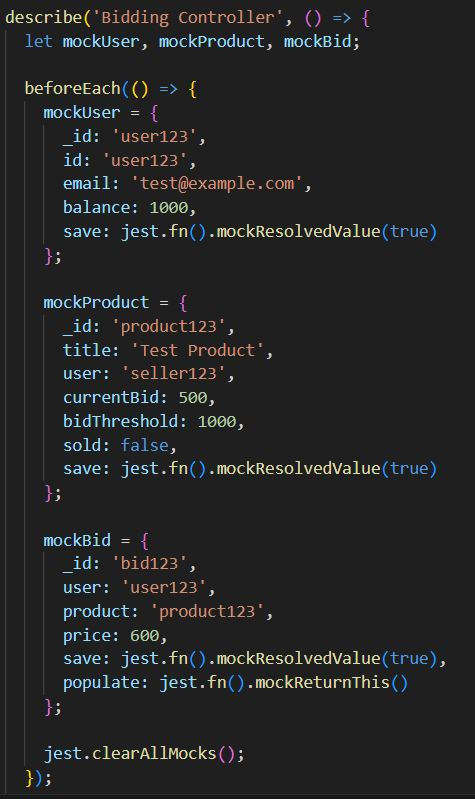
\includegraphics[width=0.5\textwidth]{Diagrams/testbidding}
    \caption{Үнэ өгөх тест 1}
    \label{fig:unit-bid1}
\end{figure}
\begin{figure}[htbp]
    \centering
    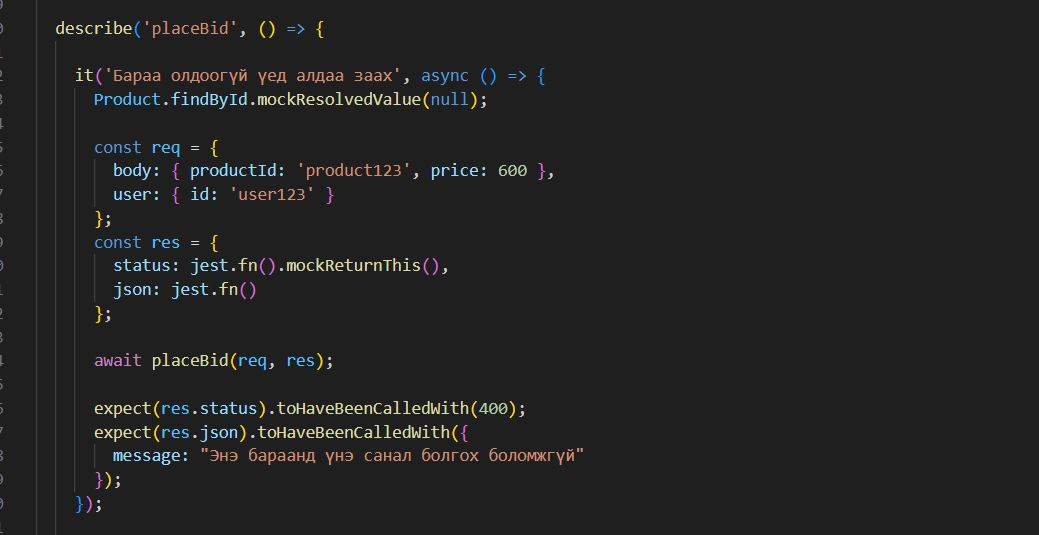
\includegraphics[scale=0.6]{Diagrams/bidtest}
    \caption{Үнэ өгөх тест 2}
    \label{fig:unit-bid2}
\end{figure}
\begin{figure}[htbp]
    \centering
    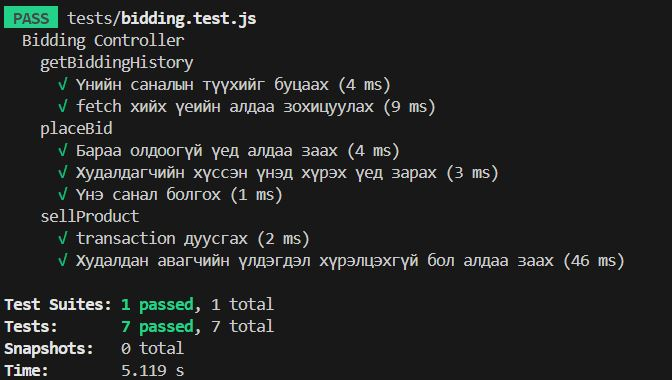
\includegraphics[width=0.7\textwidth]{Diagrams/biddingres}
    \caption{Үнэ өгөх тест хариу}
    \label{fig:unit-bidres}
\end{figure}

\clearpage
\textbf{UserController test}
\begin{figure}[htbp]
    \centering
    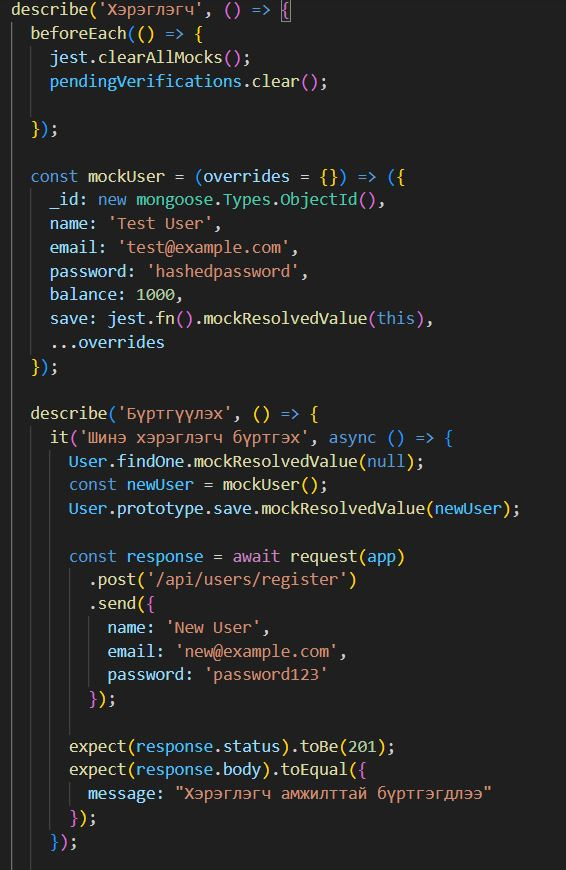
\includegraphics[width=0.7\textwidth]{Diagrams/testuser}
    \caption{Бүртгүүлэх функц}
    \label{fig:unit-user1}
\end{figure}
\begin{figure}[htbp]
    \centering
    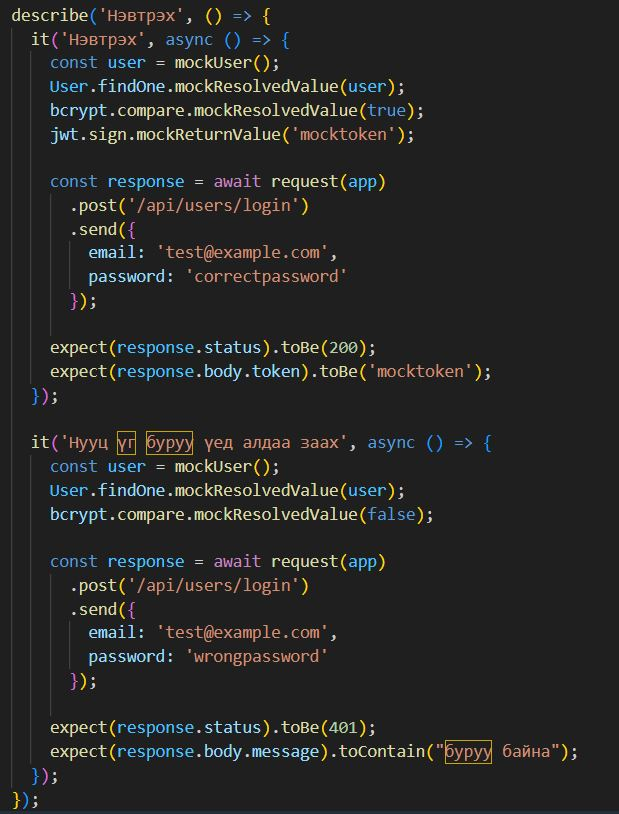
\includegraphics[width=0.5\textwidth]{Diagrams/testuser1}
    \caption{Нэвтрэх функц}
    \label{fig:unit-user2}
\end{figure}
\begin{figure}[htbp]
    \centering
    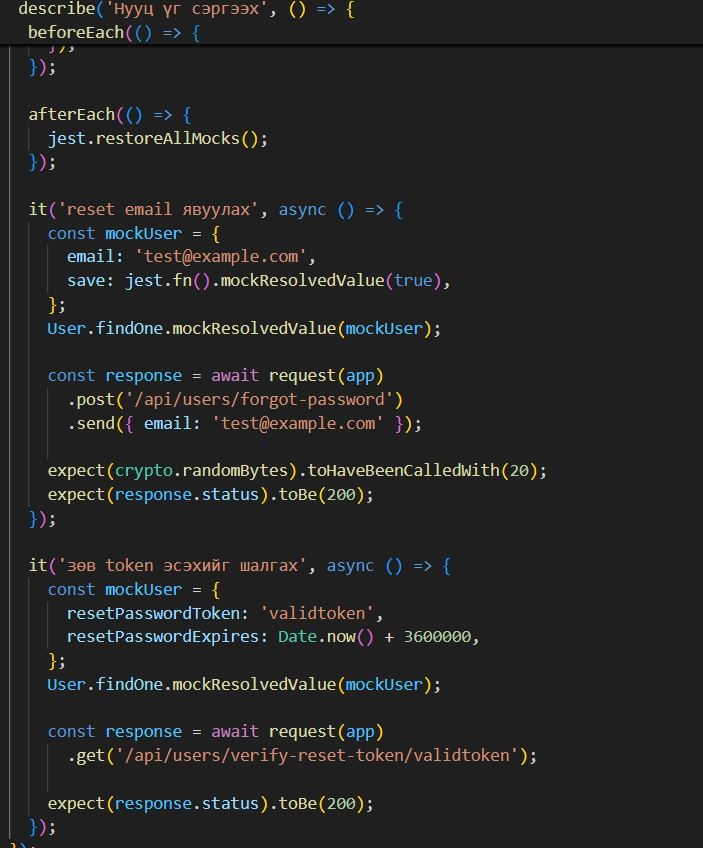
\includegraphics[width=0.5\textwidth]{Diagrams/testuser3}
    \caption{Нууц үг сэргээх функц}
    \label{fig:unit-user3}
\end{figure}


% \begin{figure}[htbp]
%     \centering
%     
\includegraphics[width=0.6\textwidth]{Diagrams/userresult}
%     \caption{Хэрэглэгчийн тестийн хариу}
%     \label{fig:unit-userres}
% \end{figure}
\newpage
\textbf{ProductController test}
\begin{figure}[htbp]
    \centering
    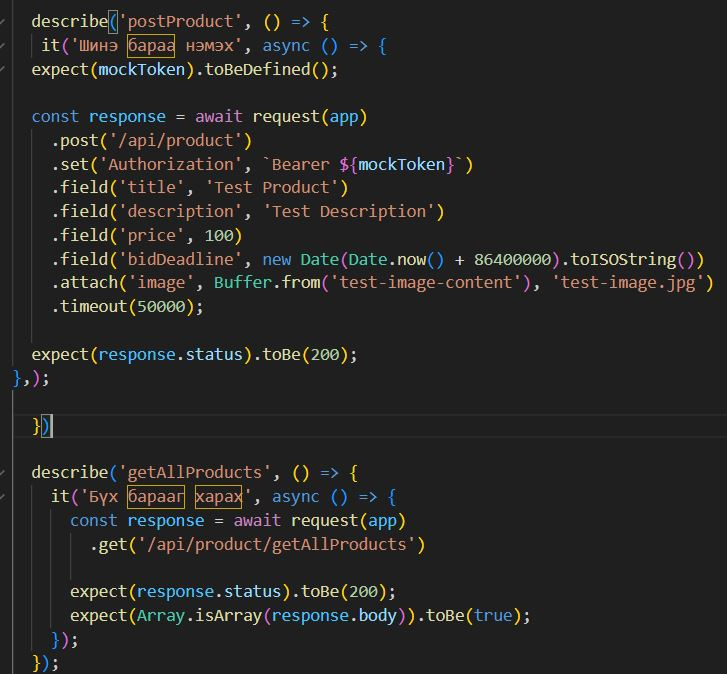
\includegraphics[width=0.7\textwidth]{Diagrams/testpro}
    \caption{Барааг нэмэх, Бараа үзэх функц}
    \label{fig:unit-product1}
\end{figure}
\begin{figure}[htbp]
    \centering
    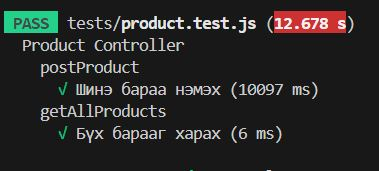
\includegraphics[width=0.7\textwidth]{Diagrams/productresult}
    \caption{Барааны тестийн хариу}
    \label{fig:unit-productres}
\end{figure}

Манай онлайн дуудлага худалдааны системд юнит тест хэрэглэх гол шалтгаанууд:

\begin{itemize}
\item Функц/модуль бүрийн зөв ажиллахыг баталгаажуулах
\item Алдааг эрт олно
\item Тест нь код хэрхэн ажиллах ёстойг харуулна
\end{itemize}
\subsection{Integration test}
Манай онлайн дуудлага худалдааны системийн үндсэн функцүүдийн хоорондын уялдаа холбоог интеграцийн тестээр шалгасан. Энэ нь:

\begin{itemize}
\item Модуль хоорондын интерфейс зөв ажиллах
\item Өгөгдлийн урсгал бүрэн бүтэн байх
\item Алдааны тохиолдолд зохих мессеж буцаах
\end{itemize}
\begin{figure}[htbp]
    \centering
    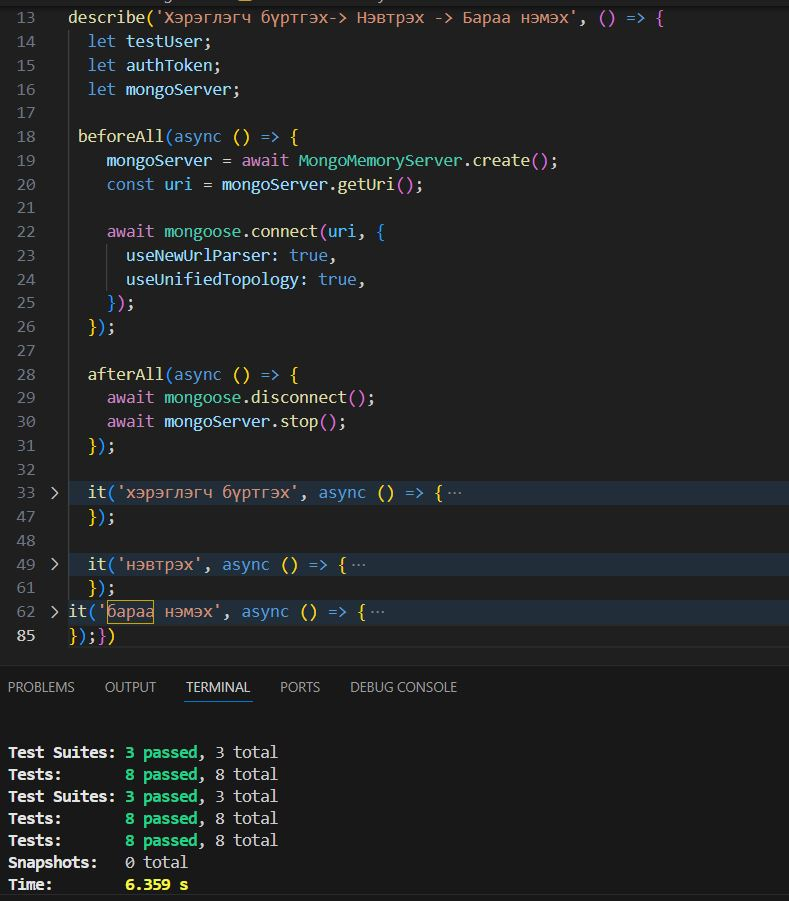
\includegraphics[width=0.7\textwidth]{Diagrams/addproductinteg.JPG}
    \caption{Бараа нэмэх функийн интеграци}
\end{figure}
\begin{figure}[htbp]
    \centering
    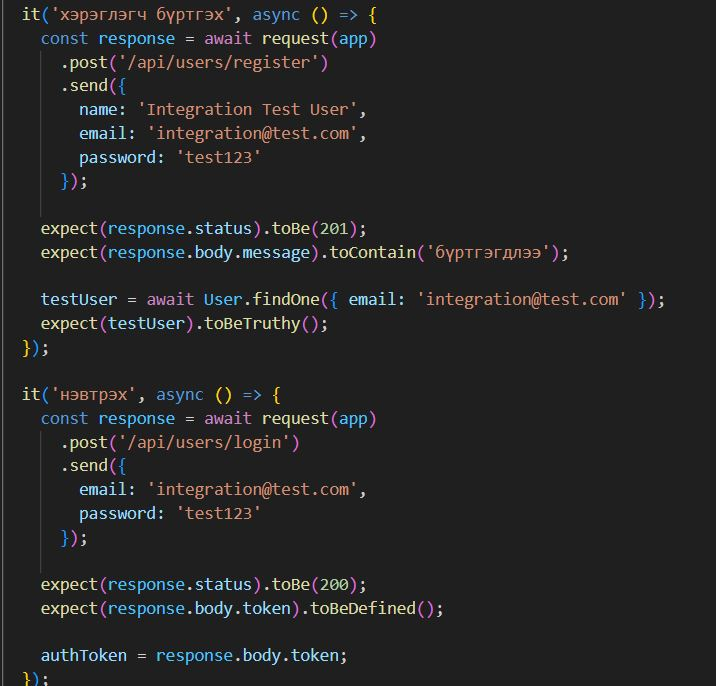
\includegraphics[width=0.7\textwidth]{Diagrams/integ}
    \caption{Хэрэглэгч бүртгүүлэх нэвтрэх функууд }

\end{figure}
\begin{figure}[htbp]
    \centering
    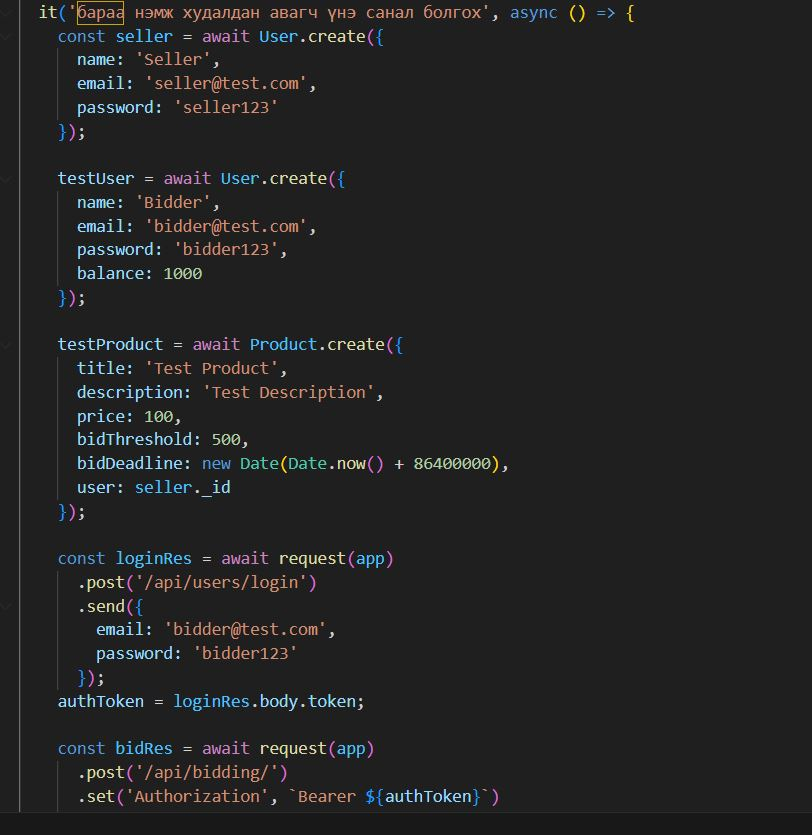
\includegraphics[width=0.7\textwidth]{Diagrams/placebidint}
    \caption{Үнэ өгөх функцийн интеграци 1}
\end{figure}
\begin{figure}[htbp]
    \centering
    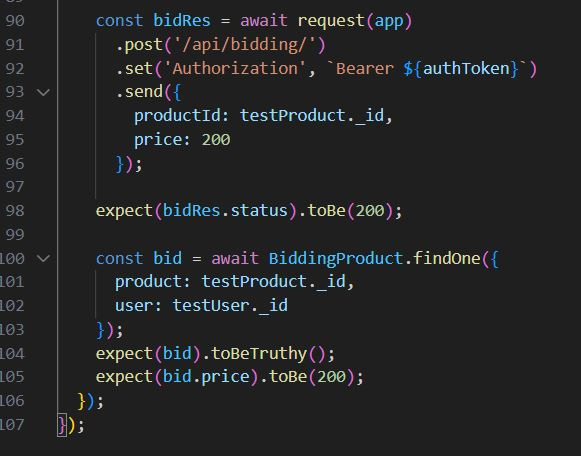
\includegraphics[width=0.7\textwidth]{Diagrams/placebidint2}
    \caption{Үнэ өгөх функцийн интеграци 2}
\end{figure}
\clearpage

\subsection{Мобайл аппликейшны тест}
Мобайл аппликейшныг дараах төрлийн тестүүдээр шалгасан:

\subsubsection{Expo Go ашиглан тест}
Хөгжүүлэлтийн явцад Expo Go аппликейшн ашиглан бодит төхөөрөмж дээр тест хийсэн:
\begin{figure}[htbp]
    \centering
    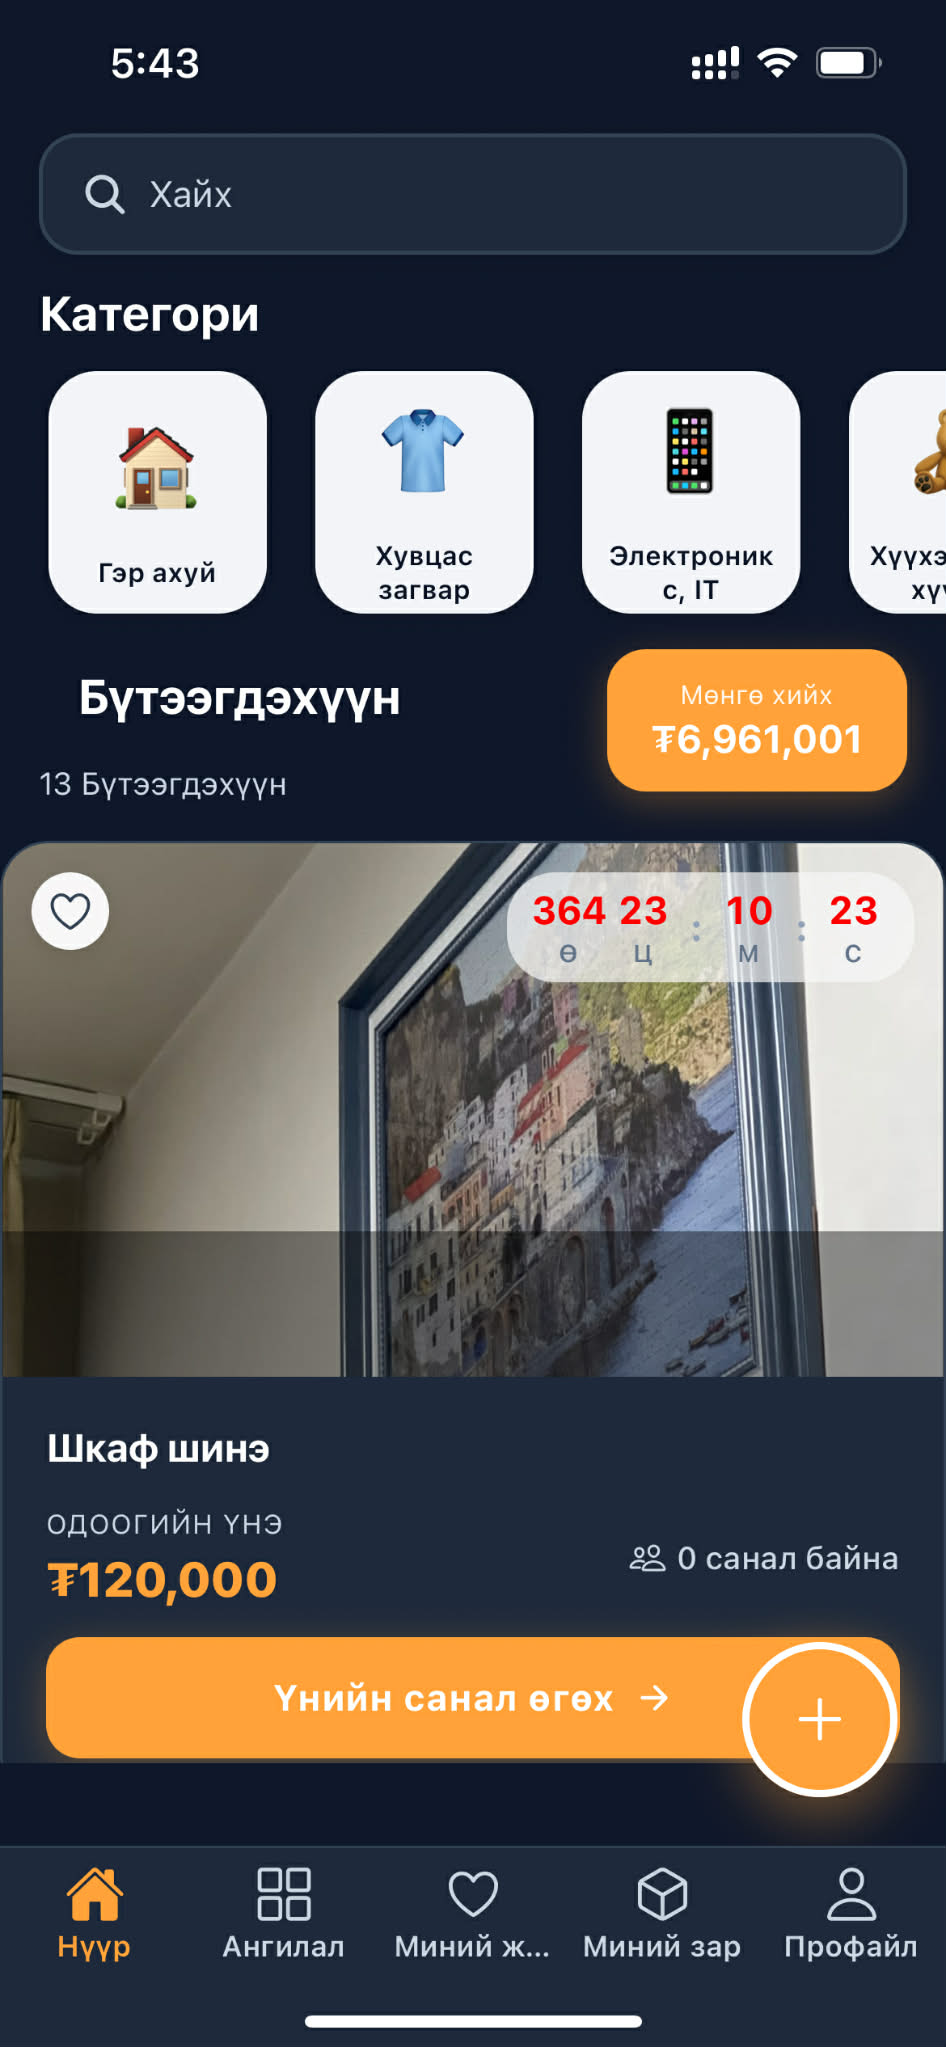
\includegraphics[width=0.5\linewidth]{ss/home.jpg}
    \caption{iOS үйлдлийн систем дээрх дэлгэц}
    \label{fig:mobile-home}
\end{figure}
\begin{itemize}
\item iOS төхөөрөмж дээр тест
\item Android төхөөрөмж дээр тест
\item QR код scan хийж шуурхай тест хийх
\item Hot reload ашиглан өөрчлөлтийг шууд харах
\end{itemize}

\subsubsection{Функциональ тест}
Мобайл аппликейшны үндсэн функцууд:
\begin{itemize}
\item \textbf{Нэвтрэх систем}: Google OAuth, утасны дугаараар баталгаажуулалт
\item \textbf{Бараа нэмэх}: Зураг оруулах, категори сонгох, мэдээлэл бөглөх
\item \textbf{Дуудлага худалдаа}: Үнэ санал болгох, real-time шинэчлэлт
\item \textbf{Хайлт, шүүлтүүр}: Барааны хайлт, категориор шүүх
\item \textbf{Профайл}: Хэрэглэгчийн мэдээлэл засах, balance харах
\end{itemize}
\begin{figure}[htbp]
    \centering
    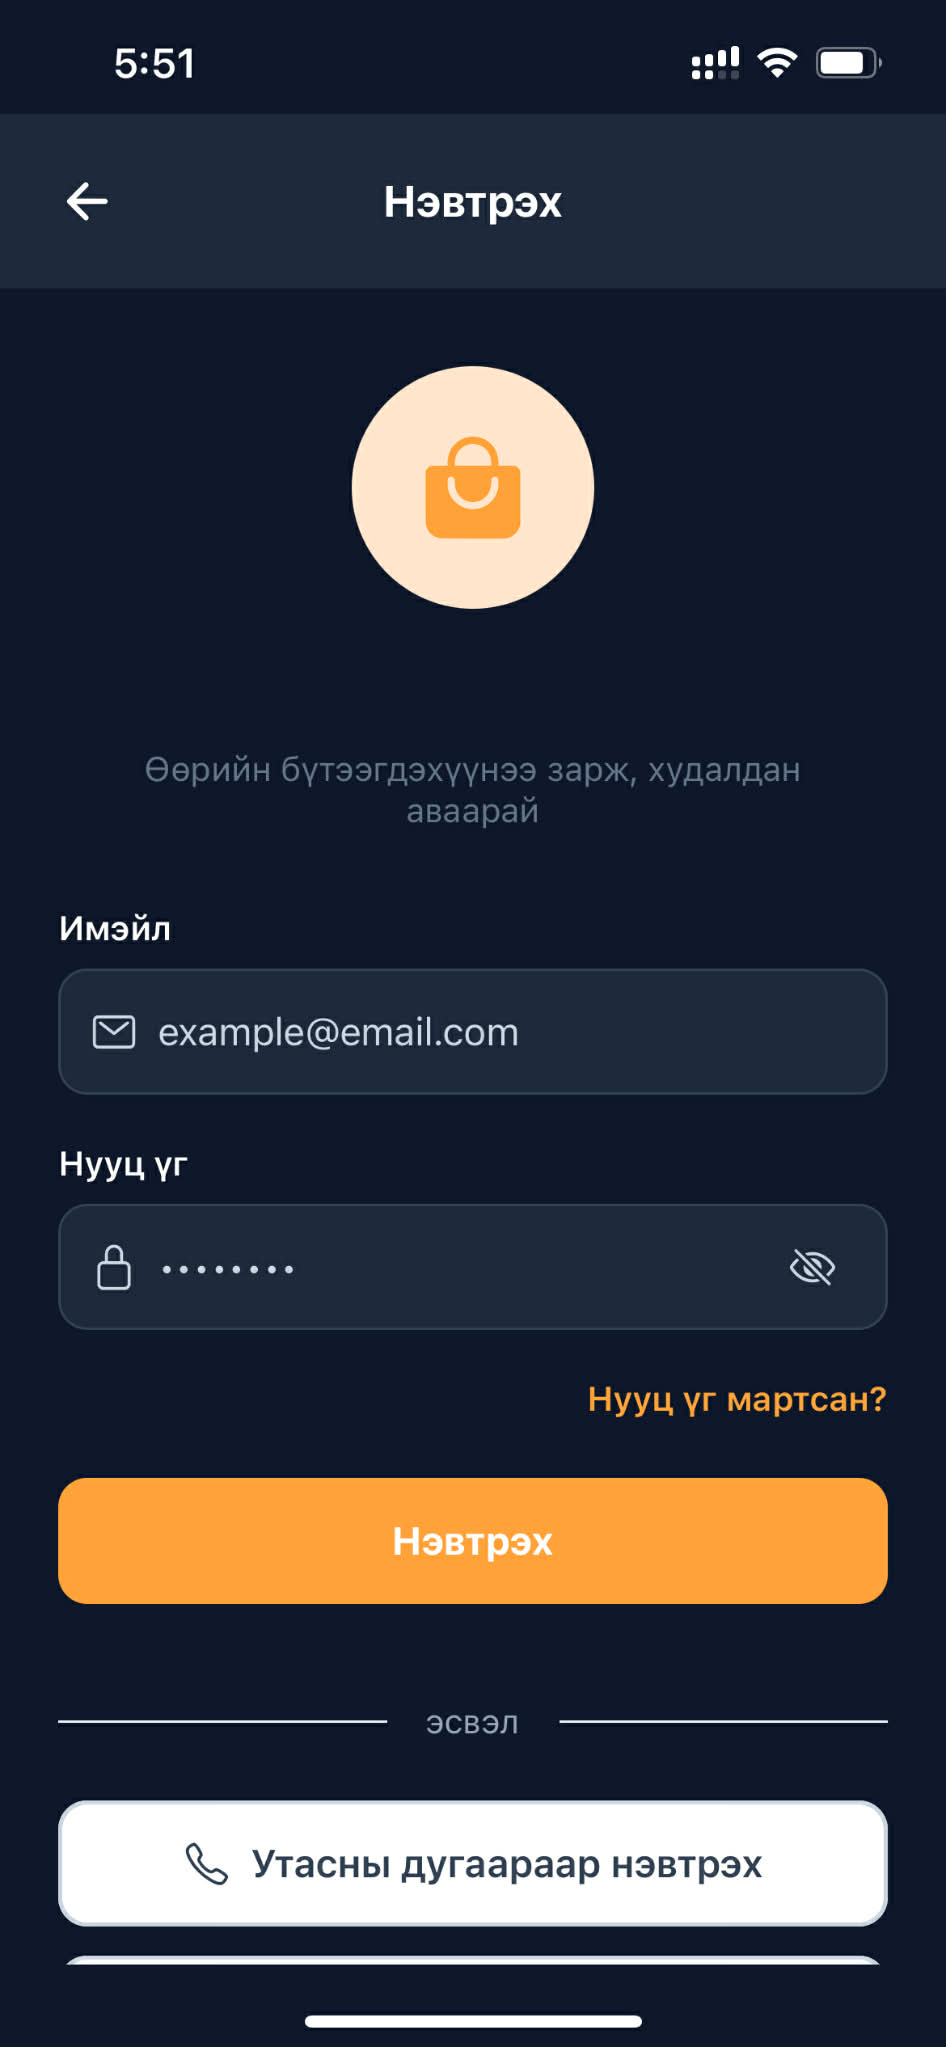
\includegraphics[width=0.3\linewidth]{ss/login screen.jpg}
    \caption{Нэвтрэх дэлгэц}
    \label{fig:mobile-login}
\end{figure}
\begin{figure}[htbp]
    \centering
    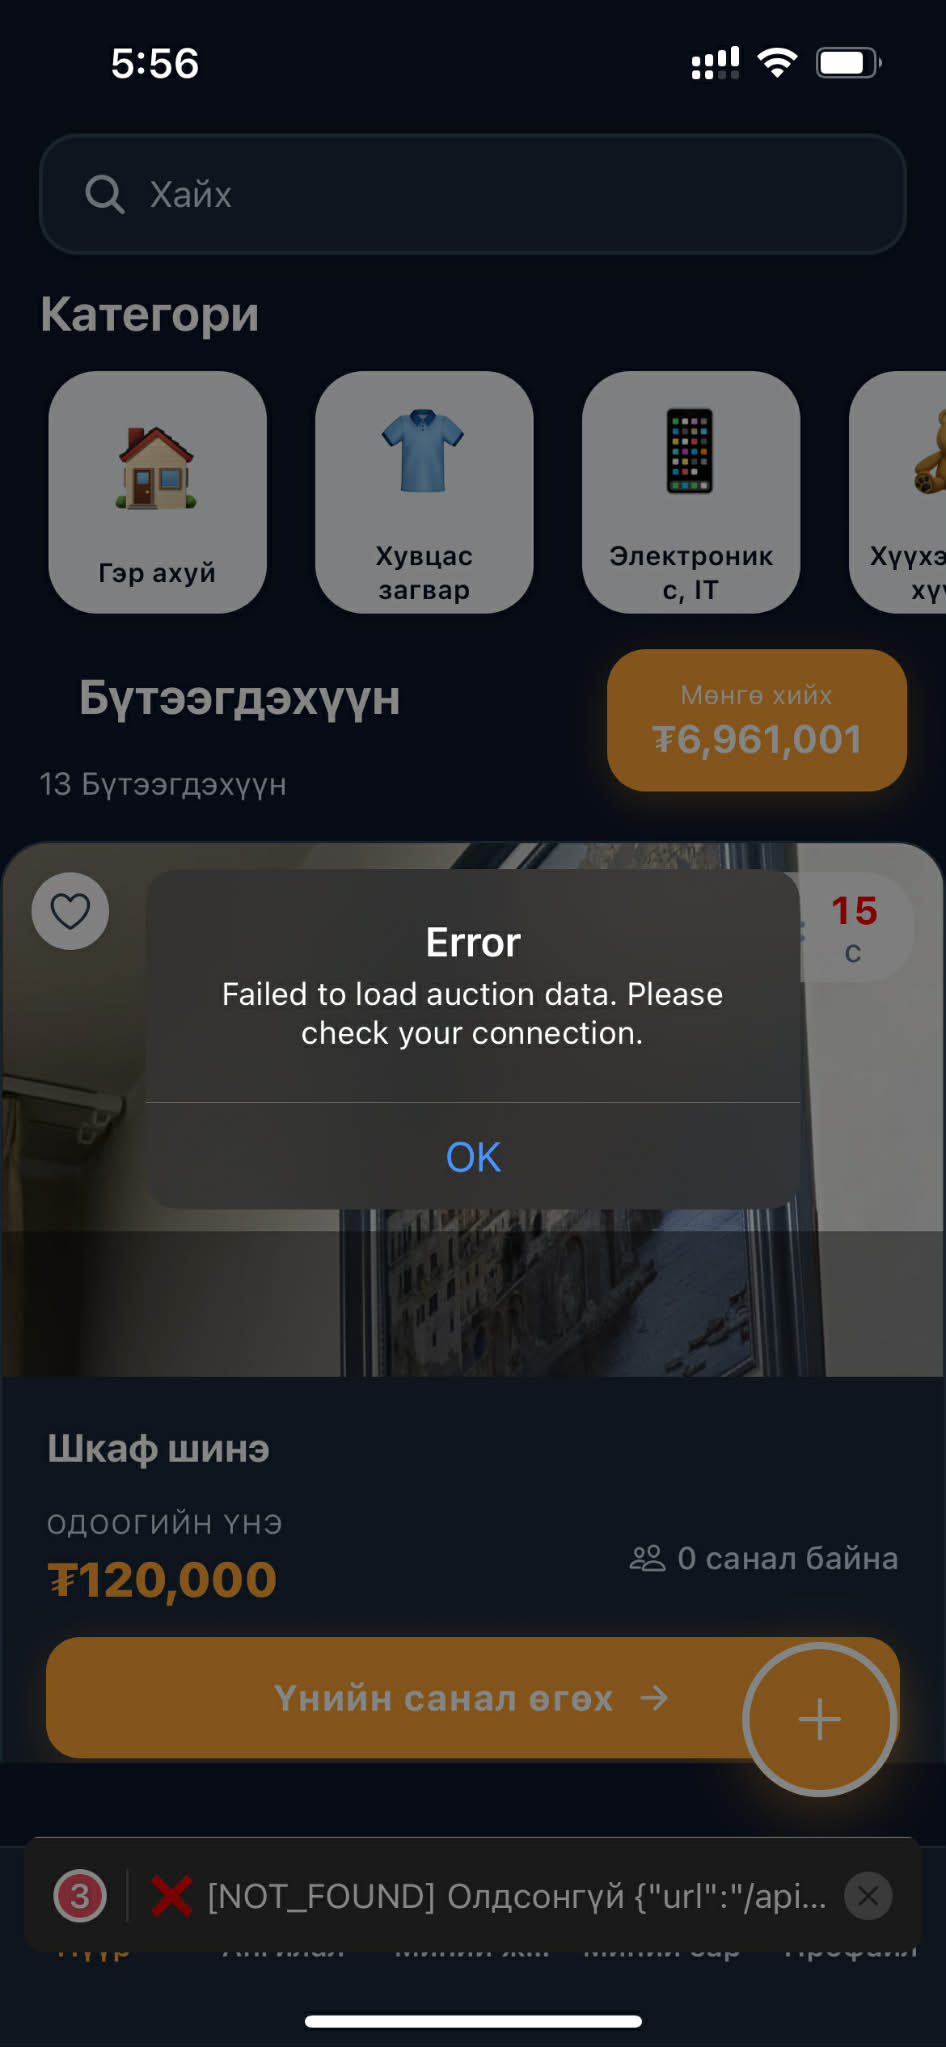
\includegraphics[width=0.3\linewidth]{ss/network error.jpg}
    \caption{Интернет холболт тасарсан үед}
    \label{fig:mobile-neterror}
\end{figure}

\subsubsection{Платформ хоорондын тест}
Дараах төхөөрөмжүүд дээр ажиллагааг шалгасан:
\begin{itemize}
\item iPhone (iOS 14+)
\item Android утас (Android 11+)
\item Tablet төхөөрөмжүүд
\item Өөр өөр дэлгэцийн хэмжээнүүд
\end{itemize}

\subsubsection{Network тест}
\begin{itemize}
\item ngrok ашиглан орон нутгийн серверт холбогдох
\item API endpoint-үүдийн хариу харах
\item Socket.io real-time холболт шалгах
\item Интернет холболт тасарсан үед алдааны харуулалт
\end{itemize}
\begin{figure}[htbp]
    \centering
    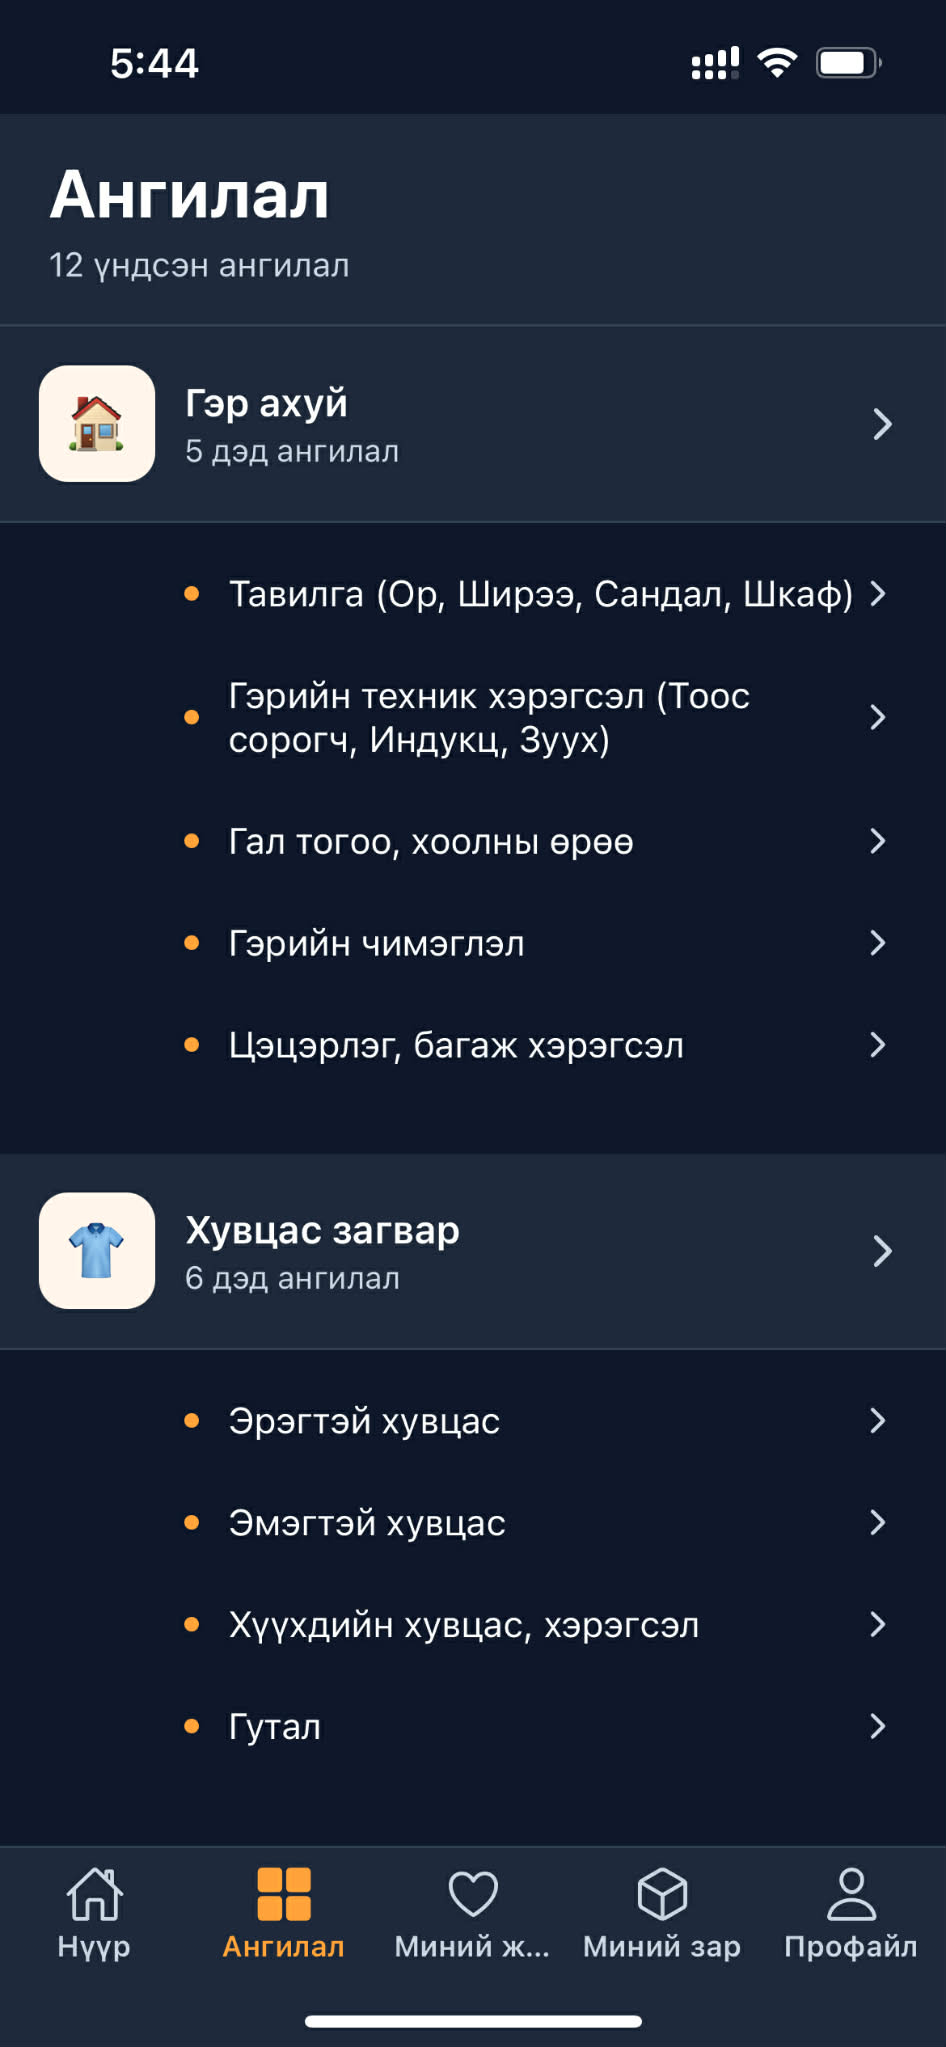
\includegraphics[width=0.3\linewidth]{ss/categories.jpg}
    \caption{Категори}
    \label{fig:mobile-categories}
\end{figure}
\subsubsection{UI/UX тест}
\begin{figure}[htbp]
    \centering
    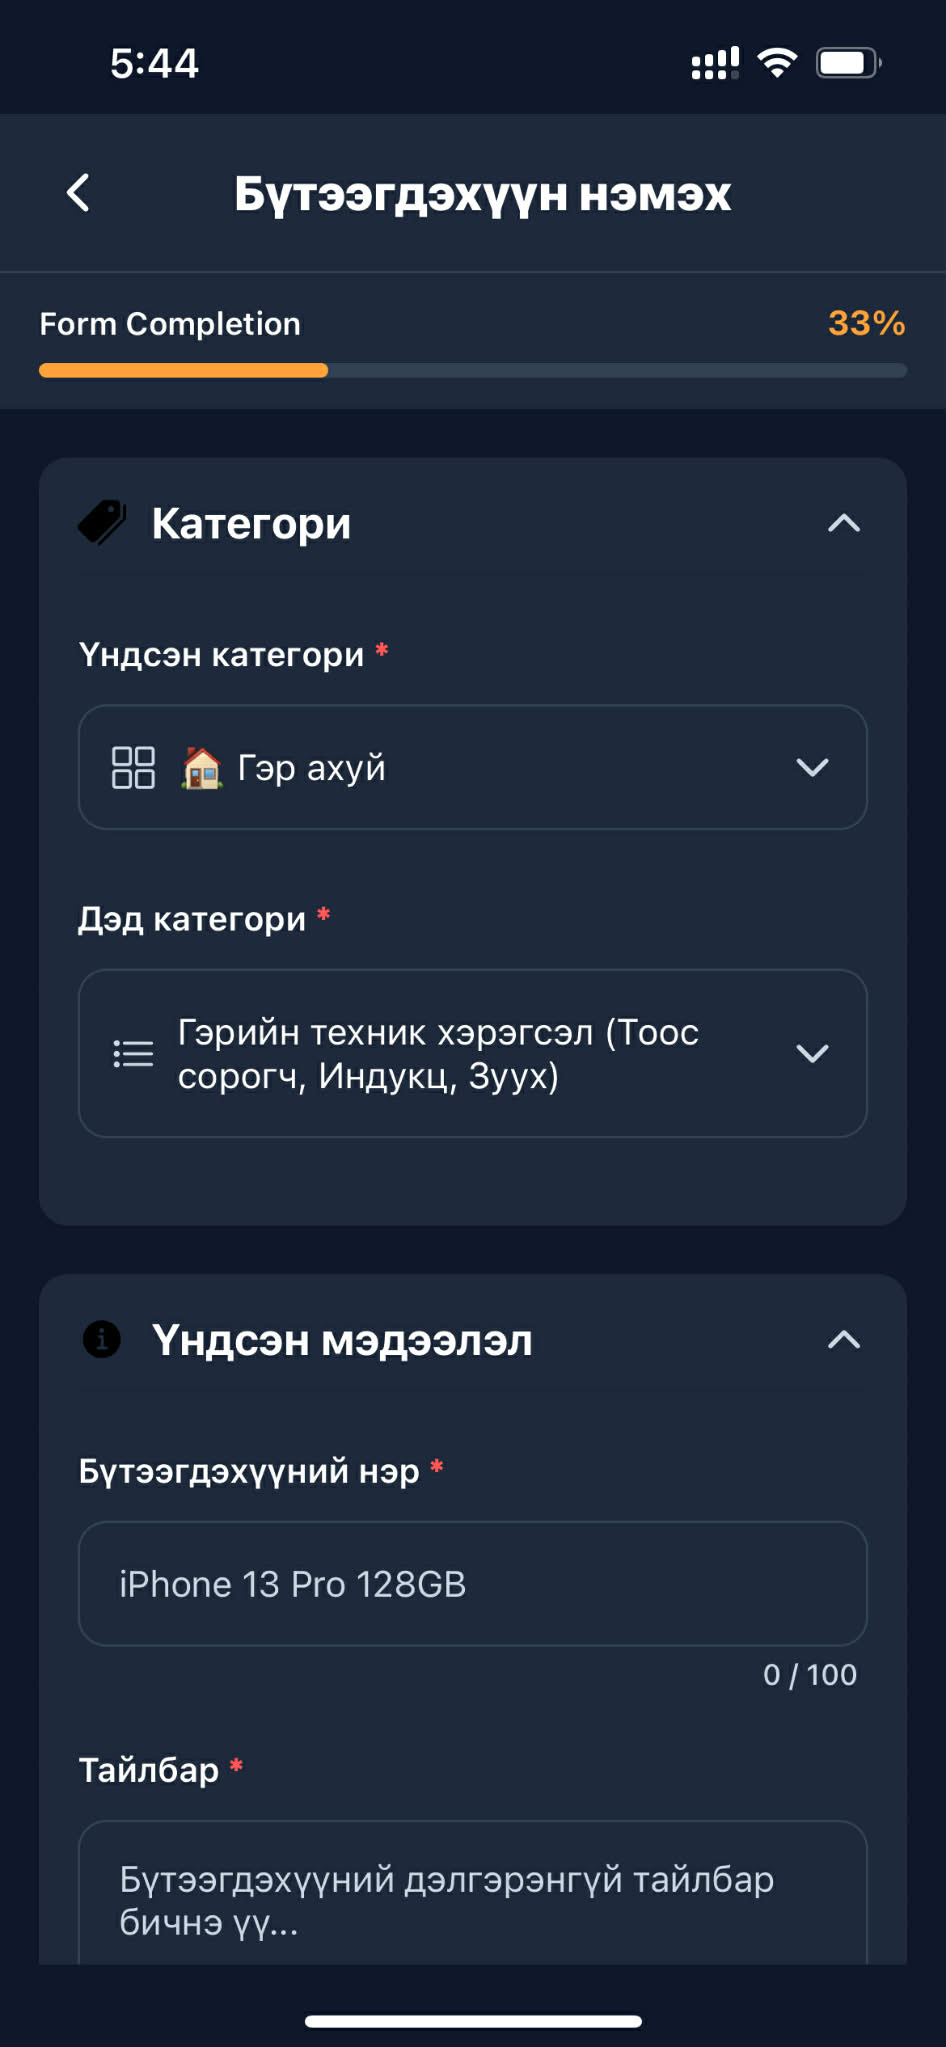
\includegraphics[width=0.3\linewidth]{ss/add product category.jpg}
    \caption{Категори сонгосон байгаа байдал}
    \label{fig:mobile-addcategory}
\end{figure}
\begin{itemize}
\item Монгол хэл дэмжлэг шалгах
\item Навигаци хялбар байх
\item Loading states харуулах
\item Error messages тодорхой байх
\item Touch targets хангалттай том байх (44x44 pixels)
\end{itemize}

\subsection{Front-End буюу админ панел}


\begin{figure}
    \centering
    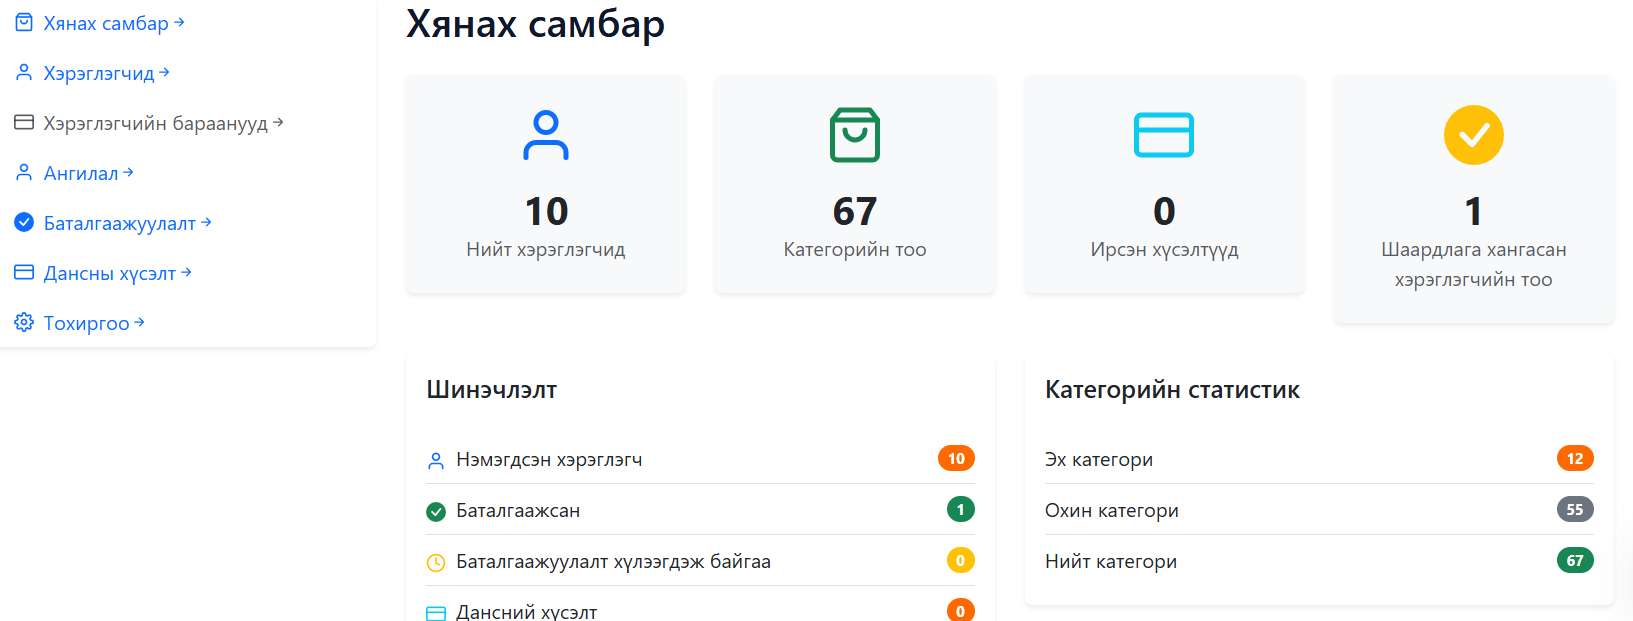
\includegraphics[width=1\linewidth]{ss/Screenshot 2025-12-25 060418.png}
    \caption{Админ панел}
\end{figure}
\subsection{Системийн үр дүн}
Хөгжүүлсэн онлайн дуудлага худалдааны систем нь:
\begin{itemize}
\item \textbf{3 платформ}: Web (React.js), Mobile (React Native), Backend (Node.js)
\item \textbf{66 категори}: Монгол зах зээлд зориулсан категориуд
\item \textbf{Real-time систем}: Socket.io ашиглан бодит цагийн дуудлага худалдаа
\item \textbf{Олон төрлийн нэвтрэх}: Google, утасны дугаар, и-мэйл
\item \textbf{Аюулгүй байдал}: JWT токен, bcrypt шифрлэлт
\item \textbf{Төлбөрийн систем}: QPay интеграци
\item \textbf{Мэдэгдлийн систем}: Firebase Cloud Messaging
\end{itemize}

\subsection{Гүйцэтгэлийн үр дүн}
Системийн гүйцэтгэл:
\begin{itemize}
\item Хуудас ачаалах хугацаа: 2-3 секунд
\item API хариу өгөх хугацаа: 200-500ms
\item Real-time үнийн шинэчлэлт: < 1 секунд
\item Зураг ачаалах: Cloudinary CDN ашиглан хурдан
\item Мобайл апп хэмжээ: ~50MB (Expo)
\end{itemize}

\clearpage